\documentclass[10pt]{article}

% -------------------------------------------------------
% PACKAGES
% -------------------------------------------------------
\usepackage[T1]{fontenc}
\usepackage[utf8]{inputenc}
\usepackage{lmodern}
\usepackage[english]{babel}
\usepackage{microtype}
\usepackage{geometry}
\geometry{
  a4paper,
  top=2.5cm, bottom=2.5cm,
  left=3cm, right=3cm
}
\usepackage{amsmath,amssymb}
\usepackage{graphicx}
\usepackage{booktabs}
\usepackage{array}
\usepackage{xcolor}
\usepackage{hyperref}
\hypersetup{
  colorlinks=true,
  linkcolor=black,
  citecolor=black,
  urlcolor=blue
}
\usepackage{caption}
\captionsetup{font=small, labelfont=bf, skip=4pt}
\usepackage{abstract}
\renewcommand{\abstractnamefont}{\normalfont\bfseries}
\renewcommand{\abstracttextfont}{\normalfont\small}
\usepackage{titlesec}
\titleformat{\section}{\normalfont\large\bfseries}{\thesection}{0.5em}{}
\titleformat{\subsection}{\normalfont\normalsize\bfseries}{\thesubsection}{0.5em}{}
\titleformat{\subsubsection}{\normalfont\normalsize\itshape}{\thesubsubsection}{0.5em}{}
\titlespacing{\section}{0pt}{8pt}{4pt}
\titlespacing{\subsection}{0pt}{6pt}{3pt}
\usepackage{parskip}
\setlength{\parskip}{4pt}
\setlength{\parindent}{0pt}
\usepackage{cite}
\usepackage{url}
\usepackage{float}
\usepackage{enumitem}
\setlist{noitemsep, topsep=2pt}

% -------------------------------------------------------
% TITLE
% -------------------------------------------------------
\title{
  \vspace{-0.5cm}
  {\large \textsc{Portfolio Research Project}} \\[0.4em]
  {\LARGE \textbf{Cinematic Speech as a Stress Test\\
  for Facial Animation Systems}} \\[0.4em]
}

\author{
  \textbf{Alex Argese} \\
  \small MSc Data Science Engineering, EURECOM \\
  \small MSc Digital Media Engineering, Politecnico di Torino \\
  \small \texttt{argesealex@gmail.com}
}

\date{\small April 2026; methodology revision November 2026}

% -------------------------------------------------------
% DOCUMENT
% -------------------------------------------------------
\begin{document}

\maketitle
\thispagestyle{plain}

% -------------------------------------------------------
% ABSTRACT
% -------------------------------------------------------

\begin{abstract}
Speech-driven facial animation must capture expression as well as articulation.
This exploratory report compares a curated Disney Cinematic Corpus (DCC) of 73
dialogues against VOCASET using text emotion classification, and inspects facial
motion with two separate pipelines. Historical classifier outputs label 68.5\% of
a 73-sentence VOCASET sample and 32.9\% of DCC dialogue as neutral. Agreement with
one author's context-aware annotations, mapped to seven categories, is 31.5\%.
A visual pilot examines one VOCASET/FaceFormer mesh pair and MediaPipe landmarks
from five animated clips. A repository audit found unresolved temporal alignment,
inconsistent upper-face definitions and stale notebook outputs. The earlier
cross-pipeline ``8$\times$'' claim is therefore withdrawn as a calibrated effect
size. The observations motivate cinematic dialogue as a candidate stress test,
but do not establish a general model failure or its cause. This revision clarifies
the methods and adds validation checks; it does not report new empirical runs.
\end{abstract}

\section{Introduction}
FaceFormer~\cite{faceformer} and CodeTalker~\cite{codetalker} generate 3D facial
motion from speech. VOCASET~\cite{vocaset} supplies phonetically balanced recordings,
whereas narrative dialogue can involve grief, irony and emotionally ambiguous
utterances. This motivates a question: do conventional evaluations adequately test
expressive performance on cinematic speech?

The present work is a pilot rather than a validated cinematic benchmark. Module 1
compares text emotion labels. Module 2 describes recorded mesh and landmark motion.
The experiments do not run FaceFormer on cinematic audio, train an alternative
model, or isolate the effects of training data and loss functions.

\section{Datasets and Scope}
\subsection{VOCASET}
The original notebook loads 480 transcript entries across 12 subject files and
reports 256 distinct strings after exact deduplication. These are transcript
statistics, not a measurement of the emotion in the audio or facial performances.
One 73-sentence sample is selected with \texttt{random\_state=42}. The full
deduplicated corpus should be the primary descriptive comparison; equal sample
sizes are not required to compare proportions.

\subsection{Disney Cinematic Corpus}
The DCC contains 73 dialogues selected by the author to cover diverse emotions.
Each has one fine-grained author annotation informed by narrative context. Table~\ref{tab:dcc}
follows the executable corpus in the notebook, correcting the earlier Tangled and
Moana counts. A curated sample cannot estimate emotion prevalence in cinema generally.
Exact screenplay editions and scene references remain to be documented.

\begin{table}[H]
\centering\small
\caption{DCC composition, counted from the notebook's dialogue list.}
\label{tab:dcc}
\begin{tabular}{lr}
\toprule Film & Dialogues \\\midrule
Frozen & 12 \\ Tangled & 10 \\ Coco & 12 \\ Encanto & 12 \\
Up & 11 \\ Inside Out & 8 \\ Moana & 8 \\\midrule
Total & 73 \\\bottomrule
\end{tabular}
\end{table}

\section{Module 1: Text Emotion Analysis}
\subsection{Method}
The notebook uses \texttt{j-hartmann/emotion-english-distilroberta-base}~\cite{hartmann}
and selects the largest score among neutral, joy, sadness, anger, fear, disgust and
surprise. The classifier sees isolated text; the author annotations use narrative
context. Fine-grained annotations are mapped to these seven categories (Appendix~\ref{app:mapping}).
This mapping is an interpretive choice: for example, betrayal need not imply disgust.
Agreement measures correspondence with this annotation scheme, rather than
independently established classifier accuracy. No inter-annotator reliability is available.

The revised notebook rejects unmapped labels before scoring and exports sentences,
predictions, sampled rows, the mapping, package versions and the resolved model revision.
Input files are now sorted. The original notebook used filesystem order, so seed 42
alone cannot reconstruct the historical sample; rerunning may change its percentages.

\subsection{Historical Results}
Table~\ref{tab:emotions} transcribes the stored outputs of the original notebook.
These values have not been recomputed in this revision. The full 256-string
VOCASET output reported 65.2\% neutral; the 73-string sample reported 68.5\%.
The difference illustrates why all available unique sentences should be retained
and sample sensitivity reported.

\begin{table}[H]
\centering\small
\caption{Historical classifier proportions (\%). The VOCASET column is the original size-matched sample.}
\label{tab:emotions}
\begin{tabular}{lrr}
\toprule Category & VOCASET ($n=73$) & DCC ($n=73$) \\\midrule
neutral & 68.5 & 32.9 \\ anger & 1.4 & 17.8 \\
sadness & 5.5 & 13.7 \\ fear & 4.1 & 12.3 \\
joy & 6.8 & 12.3 \\ disgust & 11.0 & 5.5 \\
surprise & 2.7 & 5.5 \\\bottomrule
\end{tabular}
\end{table}

\begin{figure}[H]
\centering
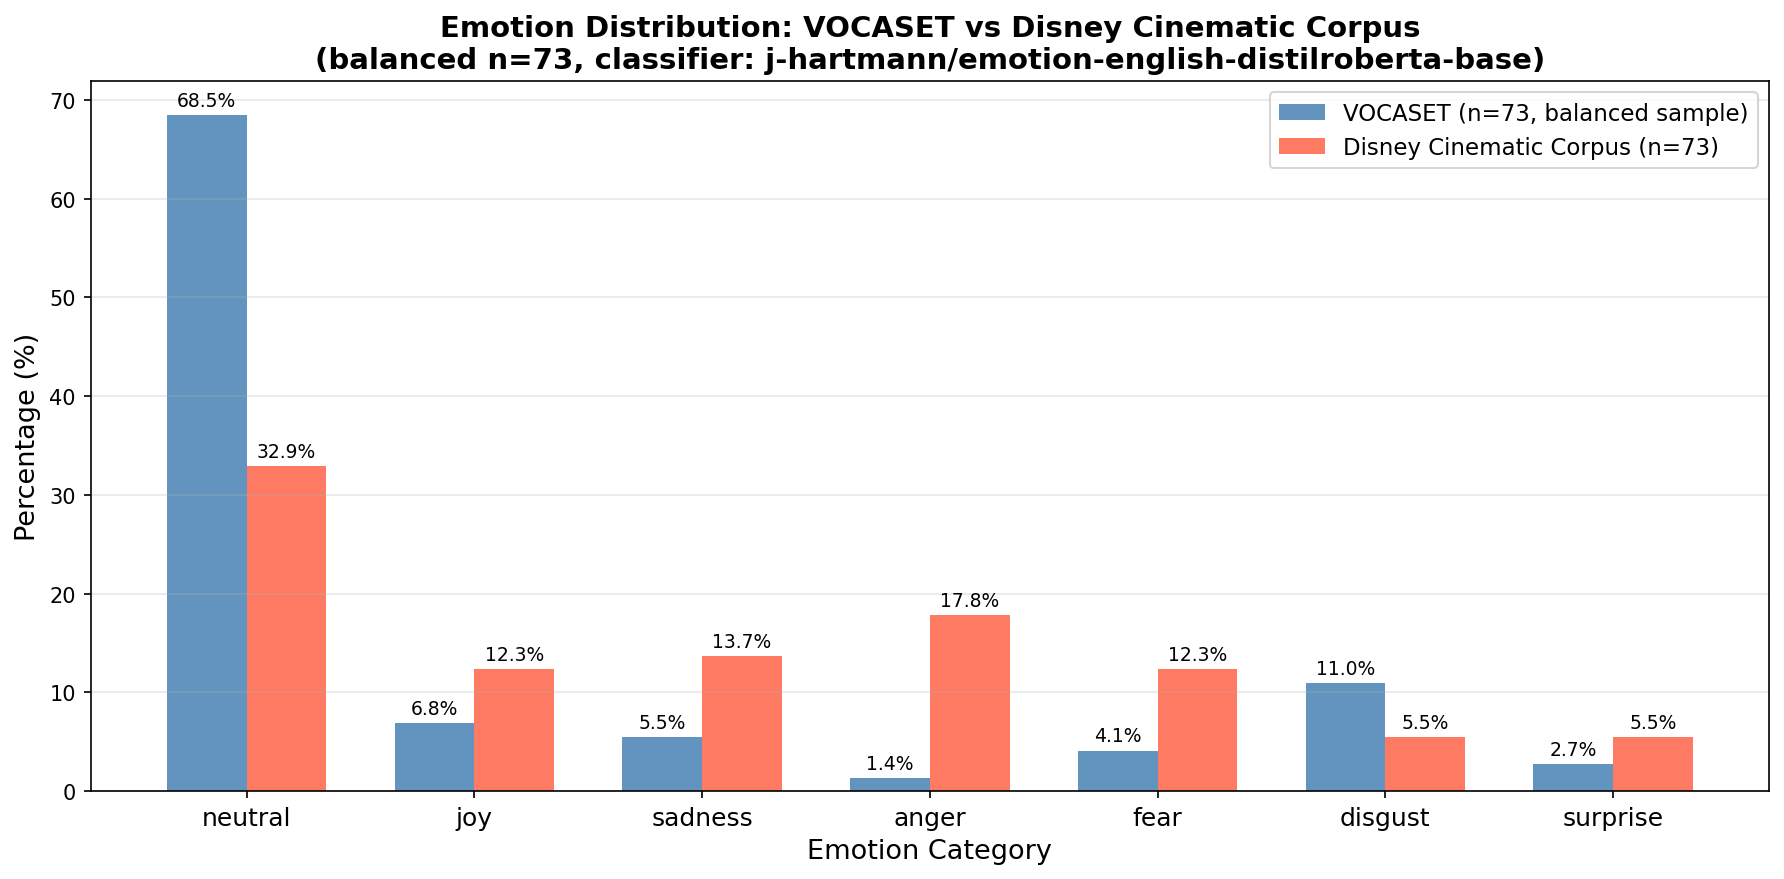
\includegraphics[width=0.92\linewidth]{figures/emotion_distribution_comparison_balanced.png}
\caption{Original classifier-distribution plot, retained as a historical result. Text labels do not establish audiovisual emotion.}
\end{figure}

Historical author--model agreement is 23/73 (31.5\%). Mapped author annotations
assign sadness to 32.9\% of dialogues, compared with 13.7\% for the classifier.
Fear and surprise have equal aggregate proportions under both labelings, but
matching proportions do not imply agreement on individual dialogues. The low overall
agreement may reflect missing context, annotation ambiguity, mapping choices,
classifier limitations, or a combination. This design does not distinguish these explanations.

\section{Module 2: Exploratory Facial Motion Analysis}
\subsection{VOCASET/FaceFormer Mesh Pair}
The original notebook loads one ground-truth and prediction pair from the
upstream evaluation repository~\cite{benchmark}.
The sequence is \texttt{FaceTalk\_170731\_00024\_TA\_sentence21}; prediction style
conditioning uses \texttt{FaceTalk\_170725\_00137\_TA}. Arrays contain 5023 XYZ
vertices per frame, with 278 ground-truth and 138 predicted frames.

\paragraph{Timing.}
The original procedure sliced both arrays to 138 frames. This does not establish
temporal alignment: a near-twofold length difference could reflect different
sampling rates or another preprocessing difference. The revised notebook requires
verified FPS values and confirmation of the same utterance and start time. It checks
durations, interpolates ground truth at prediction timestamps over shared support,
and rejects a material duration mismatch. FPS values remain unset until verified
from the actual source files and preprocessing; the revision does not assume 30 fps
for both arrays or infer rates from frame counts.

\paragraph{Regions.}
Regions use the ground-truth first frame in the original coordinate orientation,
assuming coordinates in meters:
\begin{itemize}
\item Lips: $|x|<0.035$, $-0.075<y<-0.025$, $z>-0.04$.
\item Upper face: $y>0.015$, $|x|<0.075$, $z>-0.06$.
\end{itemize}
The old executable notebook used $y>0.015$ and reported 1766 upper-face vertices;
the old paper stated $y>0.005$ and 2300 vertices. This revision follows the code's
threshold and computes region counts on execution. The geometric boxes depend on
pose, scale and coordinate conventions and require anatomical validation.

\paragraph{Statistic.}
For a region $R$, mean displacement at time $t$ is
\[
d_t^R = \frac{1000}{|R|}\sum_{v\in R}
\left\|\mathbf p_{t,v}-\mathbf p_{0,v}\right\|_2.
\]
Each sequence uses its own first frame as reference. That frame is not guaranteed
neutral. The statistic is displacement amplitude in millimeters, not inter-frame
velocity, prediction error against ground truth, or an expression-quality score.
Unremoved rigid motion can also affect it.

\paragraph{Status of earlier mesh results.}
Stored outputs report lip means of 3.870362 mm (GT) and 2.516568 mm (prediction).
However, the regional summary reports GT upper-face displacement of 0.598993 mm,
whereas a later output reports 0.578731 mm. Predicted upper-face values also differ
between the summary and the paper. These values cannot be combined as one
consistent run. The earlier ``35\%/59\% suppression'' interpretation is withheld
pending aligned execution with a fixed region definition. No replacement empirical
mesh results are claimed here.

\subsection{MediaPipe Analysis of Animated Clips}
The code extracts MediaPipe Face Landmarker~\cite{mediapipe} coordinates from
five local videos: Hans, Gothel, Miguel, Dolores and Moana. For each detected frame,
landmarks are centered on landmark 1 (nose) and divided by the distance between
landmarks 234 and 454 (cheeks). Displacement is measured relative to the first
detected frame. The lip region contains 40 landmark indices and the upper-face
region 25; the exact lists are in the notebook.

This describes the actual executable method, replacing the earlier description
of scores based on ``expected facial dynamics.'' Table~\ref{tab:clips} transcribes
stored per-clip outputs; the original videos and landmark arrays are absent from
this repository, so these results have not been independently rerun.

\begin{table}[H]
\centering\small
\caption{Historical MediaPipe outputs. Means use normalized landmark coordinates; frames count successful detections.}
\label{tab:clips}
\begin{tabular}{lrrrr}
\toprule Clip & Frames & Lip mean & Upper mean & Upper/lip \\\midrule
Hans & 100 & 0.140694 & 0.165842 & 1.178736 \\
Gothel & 177 & 0.103022 & 0.159294 & 1.546206 \\
Miguel & 123 & 0.166558 & 0.128935 & 0.774113 \\
Dolores & 217 & 0.128386 & 0.189059 & 1.472583 \\
Moana & 133 & 0.124395 & 0.136626 & 1.098324 \\\bottomrule
\end{tabular}
\end{table}

Centering and scaling do not remove head rotation, perspective changes, camera
movement, shot cuts or tracking error. The suitability of a face tracker for
stylized animated characters must be checked. A reproducible release needs clip
editions, scene timecodes, FPS, preprocessing, hashes and tracking coverage.

\subsection{Why the Earlier Eightfold Claim Is Not Established}
The historical DCC mean ratio is approximately 1.21, while a stored VOCASET
ground-truth ratio is approximately 0.15. The latter is a ground-truth statistic,
not a FaceFormer prediction statistic as stated in the original abstract.
Moreover, the two pipelines use different coordinate representations, regions
and normalization: MediaPipe landmark coordinates are not metric FLAME mesh
coordinates. Dimensionless ratios do not automatically remove these differences.
Their quotient is therefore not a calibrated estimate of cinematic motion demand.
The old cross-pipeline plots are omitted from this revision's evidence.

\section{Discussion and Next Experiments}
\paragraph{Observation versus cause.}
Differences in text labels and pilot displacement statistics motivate further work;
they do not establish that training data caused a model's behavior. The original
attribution to a lip-only LVE training objective was incorrect: the official
FaceFormer training code uses MSE over predicted vertex coordinates~\cite{ffcode}.
LVE is an evaluation metric. Controlled changes to training data and objectives
would be required to identify a cause.

\paragraph{Priority experiments.}
First, verify source timing and rerun the mesh comparison over multiple sequences,
speakers and style conditions, with sequence-level variability and anatomical
regions. Second, compare corpora in a common validated representation with head-pose
handling and tracking-quality checks. Third, run FaceFormer on the cinematic audio
itself and evaluate the output. Finally, collect independent annotations under
text-only and context-aware conditions, measuring inter-annotator agreement and
sensitivity to label mapping. These steps test separate questions and should not
be collapsed into one measure of emotional expressivity.

\section{Conclusion}
Historical text-classification outputs distinguish the selected DCC from VOCASET,
but annotation and context differences limit their interpretation. The visual pilot
contains useful extraction code and examples, while timing uncertainty, inconsistent
stored outputs and unmatched representations prevent a validated cross-corpus
effect-size claim. Cinematic dialogue remains a plausible candidate stress test.
Establishing it as a benchmark requires reproducible inputs, broader evaluation and
matched measurements. This revision provides a corrected protocol and explicit
evidence boundaries for that next stage.

\begin{thebibliography}{9}
\bibitem{vocaset}
D. Cudeiro, T. Bolkart, C. Laidlaw, A. Ranjan, and M. J. Black,
``Capture, Learning, and Synthesis of 3D Speaking Styles,'' CVPR, 2019.
\bibitem{faceformer}
Y. Fan, Z. Lin, J. Saito, W. Wang, and T. Komura,
``FaceFormer: Speech-Driven 3D Facial Animation with Transformers,'' CVPR, 2022.
\url{https://arxiv.org/abs/2112.05329}
\bibitem{codetalker}
J. Xing, M. Xia, Y. Zhang, X. Cun, J. Wang, and T.-T. Wong,
``CodeTalker: Speech-Driven 3D Facial Animation with Discrete Motion Prior,'' CVPR, 2023.
\url{https://arxiv.org/abs/2301.02379}
\bibitem{hartmann}
J. Hartmann, ``Emotion English DistilRoBERTa-base,'' 2022.
\url{https://huggingface.co/j-hartmann/emotion-english-distilroberta-base}
\bibitem{benchmark}
KAIST AMI, \texttt{Perceptual-3D-Talking-Head}, evaluation data repository.
\url{https://github.com/kaist-ami/Perceptual-3D-Talking-Head}
\bibitem{ffcode}
FaceFormer official implementation, \texttt{main.py} and \texttt{faceformer.py}.
\url{https://github.com/EvelynFan/FaceFormer}
\bibitem{mediapipe}
Google AI Edge, ``Face landmark detection guide.''
\url{https://ai.google.dev/edge/mediapipe/solutions/vision/face_landmarker}
\end{thebibliography}

\appendix
\section{Author Label Mapping}
\label{app:mapping}
The complete executable mapping is in the NLP notebook and is exported with every
run. Its main groups are reproduced below for inspection. This is a declared
annotation convention, not a validated equivalence between psychological constructs.
\begin{table}[H]
\centering\footnotesize
\begin{tabular}{p{10cm}l}
\toprule Fine-grained labels & Category \\\midrule
irony, deflection, cold, cold\_calculation, cold\_villainy, authority, wisdom,
warmth, reassurance, innocence, control, protective, determination, empathy,
protective\_love, denial, sarcasm & neutral \\\midrule
joy, excitement, tenderness, nostalgia, wonder, inspiration & joy \\\midrule
sadness, grief, melancholy, longing, regret, guilt, vulnerability, loneliness,
hidden\_pain, numbness, self\_sacrifice, heartbreak, pleading, breakdown,
inadequacy, exclusion, self\_doubt, suppressed\_sadness, emotional\_release & sadness \\\midrule
anger, defiance, frustration, repressed\_anger, injustice, confrontation & anger \\\midrule
fear, anxiety, panic, protective\_fear, desperation, repression, pressure & fear \\\midrule
disgust, manipulation, gaslighting, betrayal & disgust \\\midrule
surprise, shock, realization, inner\_conflict & surprise \\\bottomrule
\end{tabular}
\end{table}
\end{document}
